%% !TEX program = pdflatex
%% !BIB program = bibtex
\documentclass[12pt]{article}

\usepackage{amsfonts,amsmath,amssymb,mathtools,marvosym}
\usepackage[left=2.5cm,right=2cm,top=2cm,bottom=2.5cm]{geometry}
\usepackage{indentfirst,setspace,multirow}
\usepackage{graphicx,xcolor,float,epstopdf}
\usepackage{enumerate}
\usepackage[bookmarks=true,colorlinks,linkcolor=blue,citecolor=blue,urlcolor={black},breaklinks=true]{hyperref}

\usepackage{array}
\newcolumntype{P}[1]{>{\centering\arraybackslash}p{#1}}
\newcolumntype{M}[1]{>{\centering\arraybackslash}m{#1}}
\newcolumntype{N}[1]{>{\arraybackslash}m{#1}}

\onehalfspacing
%\doublespacing

\setlength{\parindent}{0.5cm}
\setlength{\parskip}{0cm}
%\renewcommand{\baselinestretch}{1.15} % 1.6 for double

% ==============================================================================

\title{\textbf{Quiz 2}}
\author{ECON312 Time Series Analysis \\ Instructor: Narek Ohanyan}
\date{}

\begin{document}

\maketitle

\vspace{1cm}

\textbf{Student} $ \qquad \underset{\text{first name}}{\underline{\hspace{4cm}}} \quad \underset{\text{last name}}{\underline{\hspace{6cm}}}  $

\bigskip
\textbf{Grade} $ \qquad \underline{\hspace{1cm}} \quad / \quad 10 $

% ------------------------------------------------------------------------------

\vspace{1cm}

\section*{Instructions}

\begin{itemize}
    \item The quiz is closed-book.
    \item No electronic devices are allowed.
    \item Write your answers in a clear and unambiguous way.

    Good luck!
\end{itemize}

% ==============================================================================

\newpage

\section*{Question 1 \normalfont{\normalsize{(10 pts.)}}}

We have following results of unit root tests for the following variables: $ W_{t} $, $ Y_{t} $, $ X_{t} $, $ Z_{t} $.

\begin{figure}[H]
    \centering
    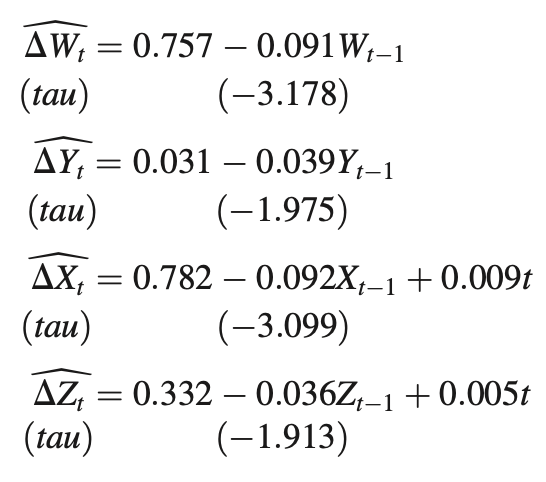
\includegraphics[width=0.4\linewidth]{fig/unit-root-equations.png}
\end{figure}

\begin{enumerate}
    \item Write down the Null and Alternative Hypotheses for the Dickey-Fuller tests above. (1 pt)
    \vspace{6cm}
    \item Sketch a graph for the distribution of the test statistic along with the rejection region(s). (1 pt)
    \vspace{6cm}
    \item Which series are stationary, and which are non-stationary at $ 95\% $ level of confidence? (6 pts)
    \vspace{15cm}
    \item Determine the order of integration for each series. (2 pts)
    \vspace{6cm}
\end{enumerate}

\begin{figure}[H]
    \centering
    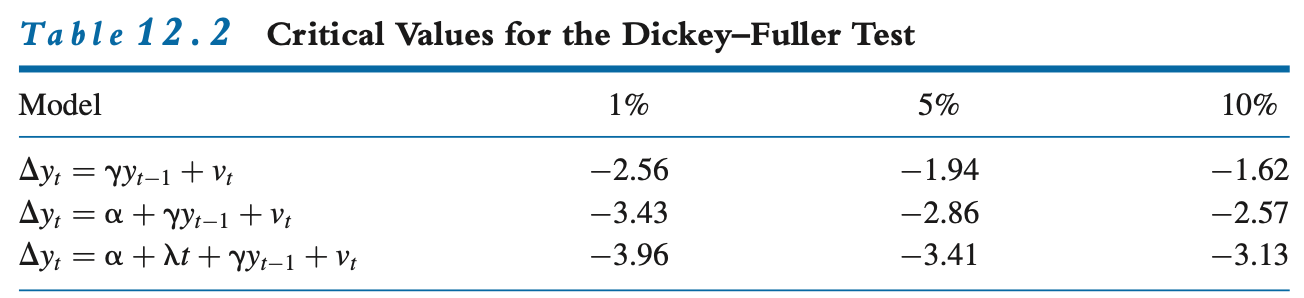
\includegraphics[width=\linewidth]{fig/critical-values.png}
\end{figure}

% =================================================================

\end{document}